\documentclass[results.tex]{subfiles}
\begin{document}

\subsection{Complete Graph}

For the Complete graph, the Graph Generator used the following parameters:

\begin{itemize}
\item Type of graph: Complete
\item Number of vertices: 20
\item Number of edges: 190
\item Random generator seed: 1615819871401
\end{itemize}
and the model took the following parameters:
\begin{itemize}
\item Total defence quota each turn: 1.0
\item Probability with which the infection propagates: 1.0
\end{itemize}

\begin{figure}[!ht]
	\centering
	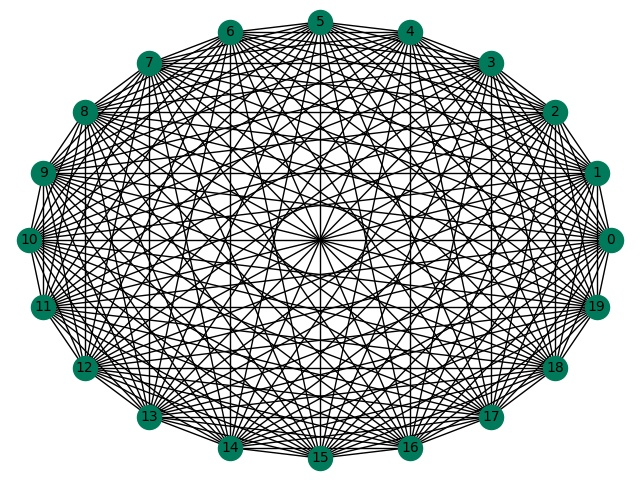
\includegraphics[width=0.9\textwidth]{complete.jpg}
	\caption{The Complete graph used.}
	\label{fig:complete}
\end{figure}

\subsubsection{Deterministic Protection}

The winning strategies by source node are listed in the table below. This really isn't too surprising - by {\it deterministic}, we mean that the initial protection is equal to the ``peril" rating of the given agent, which - in a complete graph - must be 1, since every vertex is adjacent to every other vertex and so adjacent to the source node. We can see this in the following initial agent states for source node 0:

\begin{center}
  \begin{tabular}{| c || c | c | c |}
  \hline
  Vertex Location & Peril & Protection & State\\
  \hline\hline
  0 & 1.00 & 1.00 & Infected \\
  \hline
  1 & 1.00 & 1.00 & Susceptible \\
  \hline
  2 & 1.00 & 1.00 & Susceptible \\
  \hline
  3 & 1.00 & 1.00 & Susceptible \\
  \hline
  4 & 1.00 & 1.00 & Susceptible \\
  \hline
  5 & 1.00 & 1.00 & Susceptible \\
  \hline
  6 & 1.00 & 1.00 & Susceptible \\
  \hline
  7 & 1.00 & 1.00 & Susceptible \\
  \hline
  8 & 1.00 & 1.00 & Susceptible \\
  \hline
  9 & 1.00 & 1.00 & Susceptible \\
  \hline
  10 & 1.00 & 1.00 & Susceptible \\
  \hline
  11 & 1.00 & 1.00 & Susceptible \\
  \hline
  12 & 1.00 & 1.00 & Susceptible \\
  \hline
  13 & 1.00 & 1.00 & Susceptible \\
  \hline
  14 & 1.00 & 1.00 & Susceptible \\
  \hline
  15 & 1.00 & 1.00 & Susceptible \\
  \hline
  16 & 1.00 & 1.00 & Susceptible \\
  \hline
  17 & 1.00 & 1.00 & Susceptible \\
  \hline
  18 & 1.00 & 1.00 & Susceptible \\
  \hline
  19  & 1.00 & 1.00 & Susceptible \\
  \hline
  \end{tabular}
\end{center}

Thus, all vertices become protected in the second turn as their protection rating is assigned to 1 and the model ends. In future, this would become a more interesting scenario when we introduce the notion of protection decay - the protection rating of a given agent decays over time, moving the agent back into the susceptible state.

\begin{center}
 \begin{tabular}{| c || c | c | c | c |} 
 \hline
 {\bfseries Source node} & {\bfseries Winning Strategy} & {\bfseries Infections} & {\bfseries Protections} & {\bfseries End-Turn} \\  %[0.5ex] 
 \hline\hline
 0 & All & 1 & 19 & 1 \\ 
 \hline
  1 & All & 1 & 19 & 1 \\ 
 \hline
  2 & All & 1 & 19 & 1 \\ 
 \hline
  3 & All & 1 & 19 & 1 \\ 
 \hline
  4 & All & 1 & 19 & 1 \\  
 \hline
  5 & All & 1 & 19 & 1 \\ 
 \hline
  6 & All & 1 & 19 & 1 \\  
 \hline
  7 & All & 1 & 19 & 1 \\ 
 \hline
  8 & All & 1 & 19 & 1 \\ 
 \hline
  9 & All & 1 & 19 & 1 \\ 
 \hline
 10 & All & 1 & 19 & 1 \\ 
 \hline
 11 & All & 1 & 19 & 1 \\ 
 \hline
 12 & All & 1 & 19 & 1 \\ 
 \hline
 13 & All & 1 & 19 & 1 \\ 
 \hline
 14 & All & 1 & 19 & 1 \\ 
 \hline
 15 & All & 1 & 19 & 1 \\ 
 \hline
 16 & All & 1 & 19 & 1 \\ 
 \hline
 17 & All & 1 & 19 & 1 \\ 
 \hline
 18 & All & 1 & 19 & 1 \\ 
 \hline
 19 & All & 1 & 19 & 1 \\
 \hline
 \end{tabular}
\end{center}

\newpage

\begin{figure}[!ht]
\centering
     \begin{subfigure}[b]{0.9\textwidth}
         \centering
         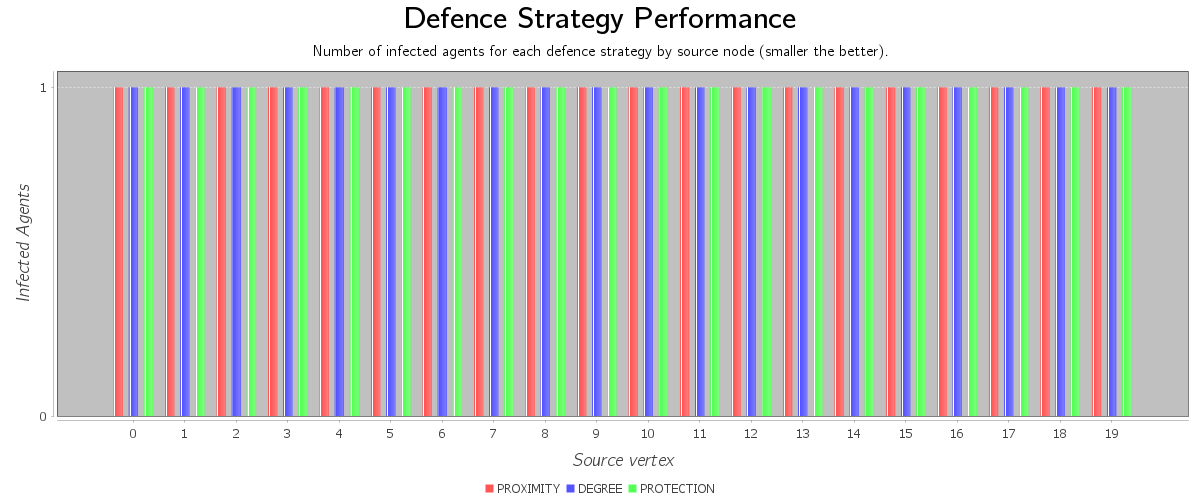
\includegraphics[width=\textwidth]{Deterministic/DeterministicInfectedChart}
         %\caption{Infected}
         \label{fig:com-det-infected}
     \end{subfigure}
     \vfill
     \begin{subfigure}[b]{0.9\textwidth}
         \centering
         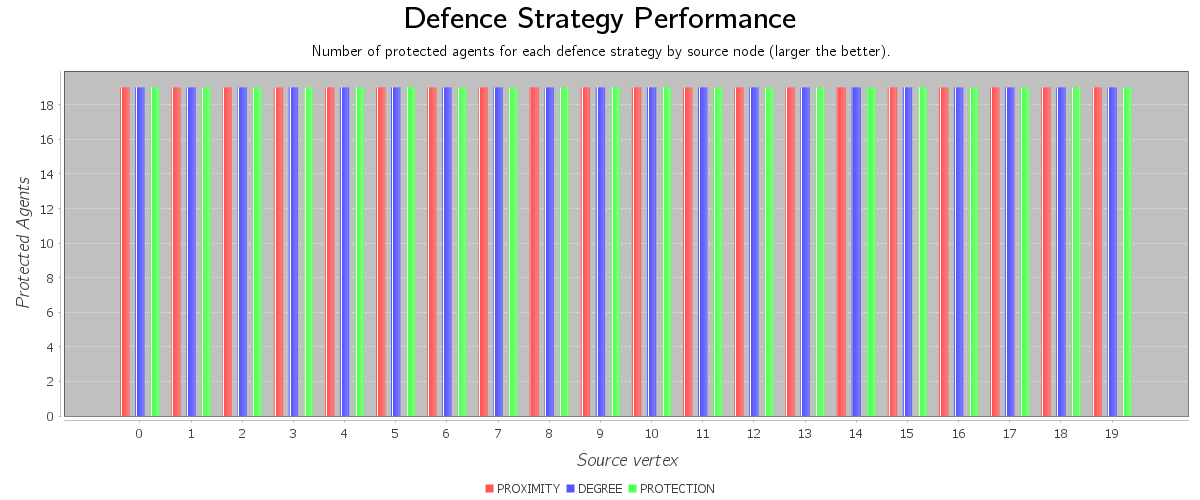
\includegraphics[width=\textwidth]{Deterministic/DeterministicProtectedChart}
         %\caption{Protected}
         \label{fig:com-det-protected}
     \end{subfigure}
     \vfill
     \begin{subfigure}[b]{0.9\textwidth}
         \centering
         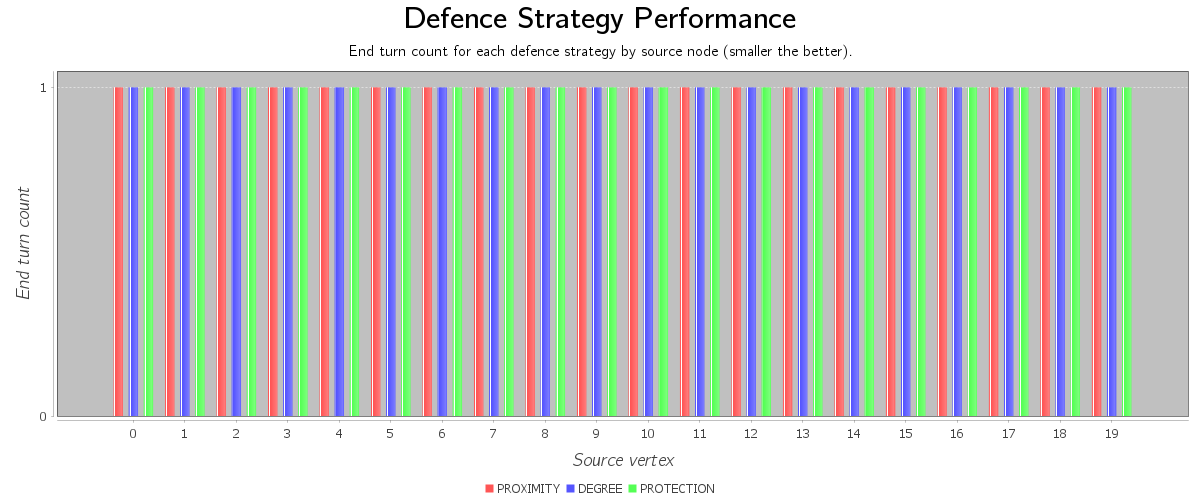
\includegraphics[width=\textwidth]{Deterministic/DeterministicEndTurnChart}
         %\caption{End Turn}
         \label{fig:com-det-end}
     \end{subfigure}
        \caption{Model results on a Complete graph by source node for each defence strategy with deterministic initial protection allocation.}
        \label{fig:com-det-charts}
\end{figure}

\newpage

\subsubsection{Mixed Protection}

Here, we allocate protection by first generating a baseline pseudo-random number and then increasing based on proximity to closest infection.

\subfile{Mixed/MixedTable.tex}

\newpage

\begin{figure}[!ht]
\centering
     \begin{subfigure}[b]{0.9\textwidth}
         \centering
         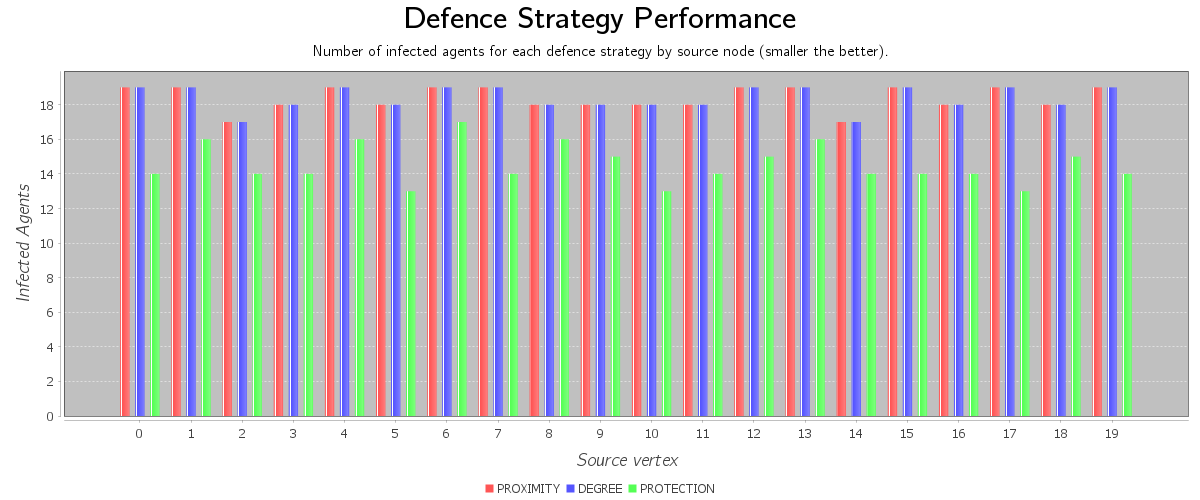
\includegraphics[width=\textwidth]{Mixed/MixedInfectedChart}
         %\caption{Infected}
         \label{fig:com-mix-infected}
     \end{subfigure}
     \vfill
     \begin{subfigure}[b]{0.9\textwidth}
         \centering
         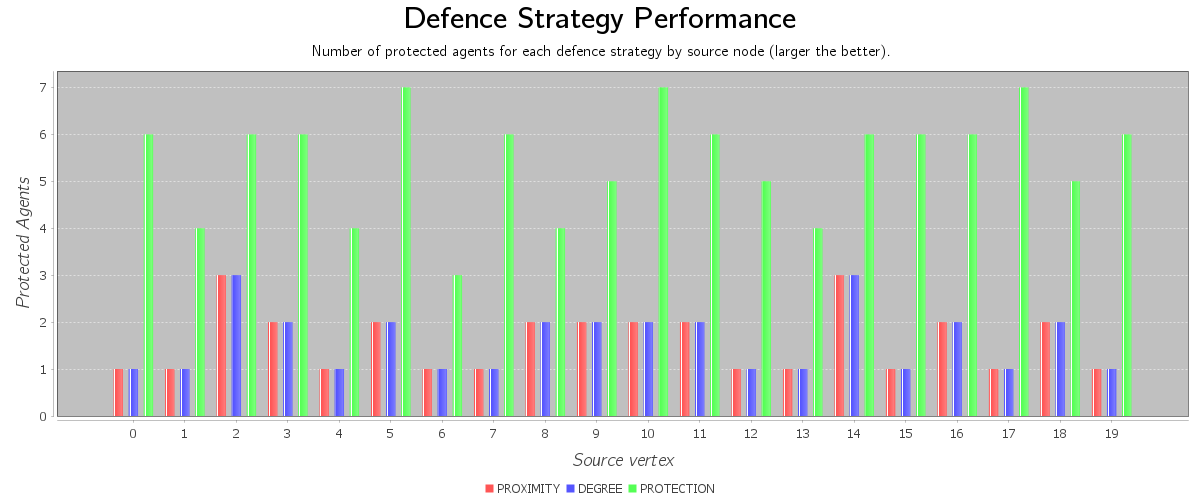
\includegraphics[width=\textwidth]{Mixed/MixedProtectedChart}
         %\caption{Protected}
         \label{fig:com-mix-protected}
     \end{subfigure}
     \vfill
     \begin{subfigure}[b]{0.9\textwidth}
         \centering
         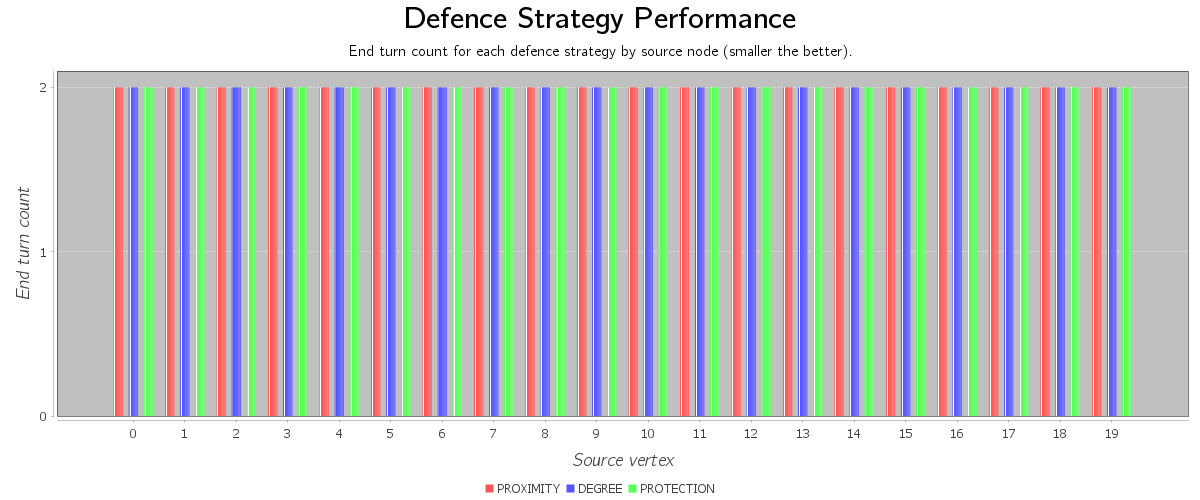
\includegraphics[width=\textwidth]{Mixed/MixedEndTurnChart}
         %\caption{End Turn}
         \label{fig:com-mix-end}
     \end{subfigure}
        \caption{Model results on a Complete graph by source node for each defence strategy with mixed initial protection allocation.}
        \label{fig:com-mix-charts}
\end{figure}

\newpage

\subsubsection{Random Protection}

Here, we generate a pseudo-random number and assigning this as the protection rating of the given vertex

\subfile{Random/RandomTable.tex}

\begin{figure}[!ht]
\centering
     \begin{subfigure}[b]{0.9\textwidth}
         \centering
         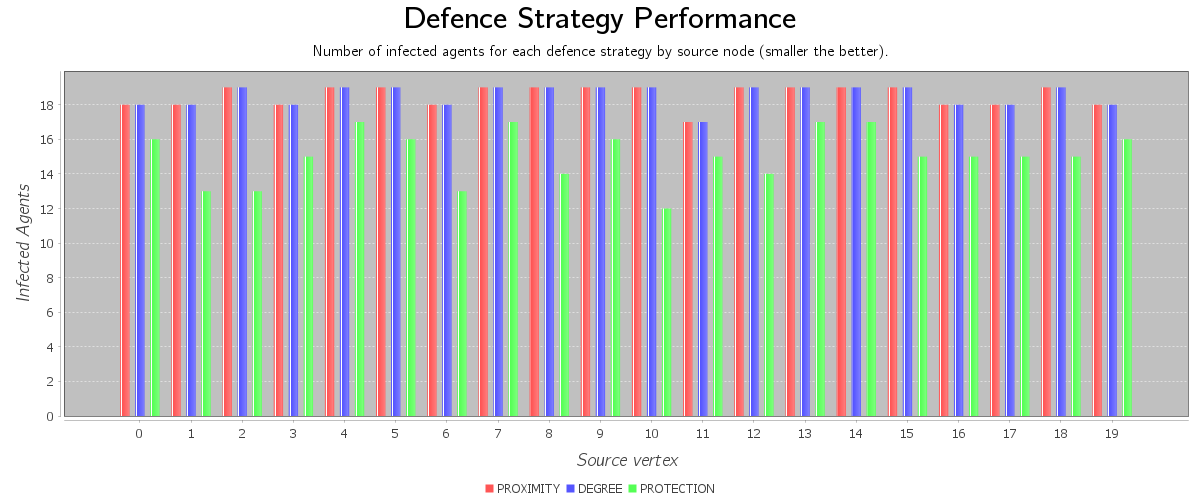
\includegraphics[width=\textwidth]{Random/RandomInfectedChart}
         %\caption{Infected}
         \label{fig:com-ran-infected}
     \end{subfigure}
     \vfill
     \begin{subfigure}[b]{0.9\textwidth}
         \centering
         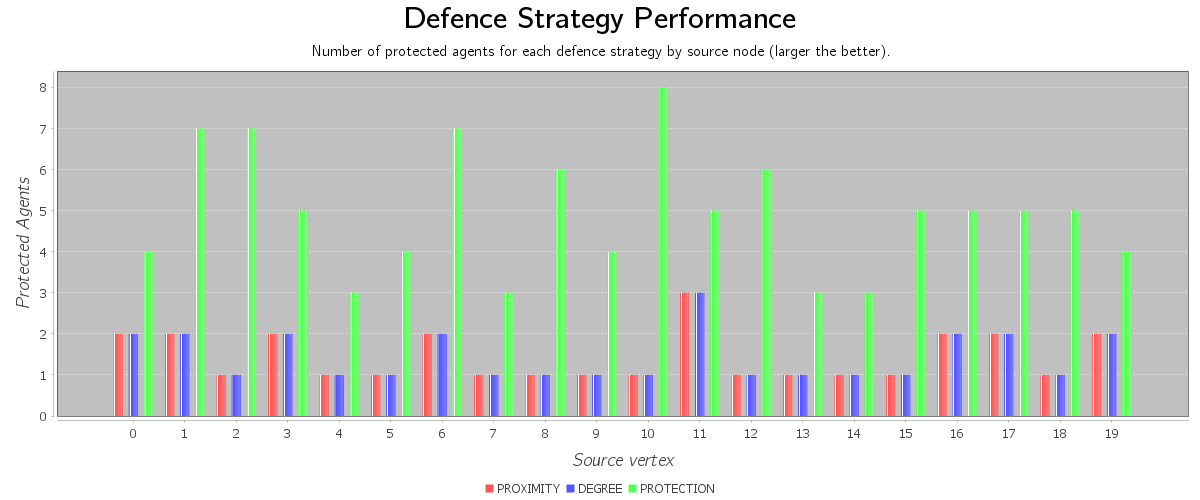
\includegraphics[width=\textwidth]{Random/RandomProtectedChart}
         %\caption{Protected}
         \label{fig:com-ran-protected}
     \end{subfigure}
     \vfill
     \begin{subfigure}[b]{0.9\textwidth}
         \centering
         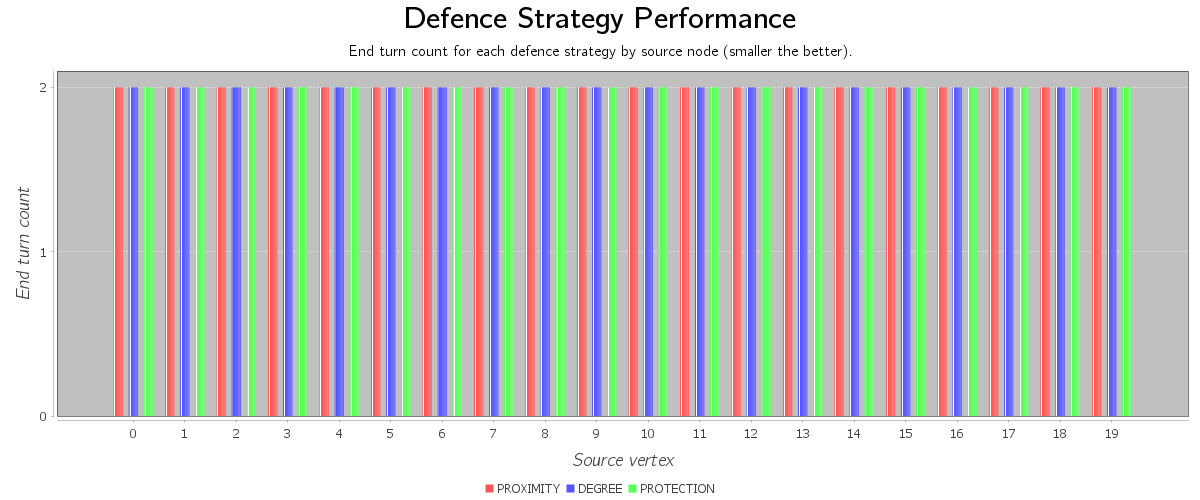
\includegraphics[width=\textwidth]{Random/RandomEndTurnChart}
         %\caption{End Turn}
         \label{fig:com-ran-end}
     \end{subfigure}
        \caption{Model results on a Complete graph by source node for each defence strategy with mixed initial protection allocation.}
        \label{fig:com-ran-charts}
\end{figure}

\end{document}